\chapter{Figures Without Layout Surprises}
\label{chap:figures}

\begin{learningoutcomes}
  \item Place a graphic with a caption and label.
  \item Create a self-contained vector diagram.
  \item Build and align two figure panels.
\end{learningoutcomes}

\section{Place your own finished graphic}

Store a graphic beside the source or in a project-relative folder:

\begin{latexcode}{Figure placement recipe}
\usepackage{graphicx}

\begin{figure}[htbp]
  \centering
  \includegraphics[width=0.78\linewidth]{figures/result.pdf}
  \caption{State what the figure shows and define its visual
  encodings.}
  \label{fig:result}
\end{figure}

Figure~\ref{fig:result} shows the main pattern.
\end{latexcode}

Use PDF for vector plots and diagrams. Use PNG or JPEG for raster material.
Set one dimension—normally the width—so the aspect ratio stays correct.

\section{Build a complete vector figure in source}

This example needs no separate image:

\begin{latexcode}{Complete example: a TikZ workflow figure}
\documentclass{article}
\usepackage{tikz}
\usetikzlibrary{arrows.meta,positioning}

\begin{document}
\begin{figure}[htbp]
  \centering
  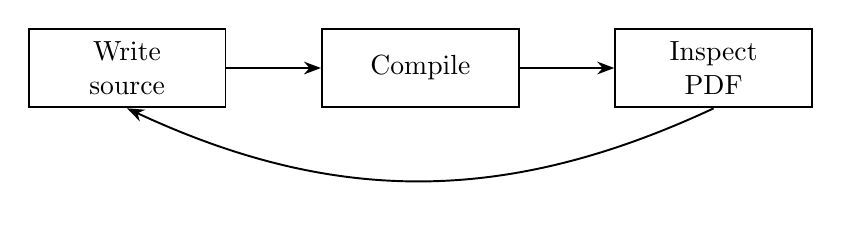
\begin{tikzpicture}[
    node distance=12mm,
    box/.style={draw,line width=.7pt,minimum width=25mm,
      minimum height=10mm,align=center},
    flow/.style={-{Stealth},line width=.7pt}
  ]
    \node[box] (source) {Write\\source};
    \node[box,right=of source] (build) {Compile};
    \node[box,right=of build] (pdf) {Inspect\\PDF};
    \draw[flow] (source) -- (build);
    \draw[flow] (build) -- (pdf);
    \draw[flow] (pdf.south) to[bend left=25] (source.south);
  \end{tikzpicture}
  \caption{The edit--compile--inspect cycle.}
  \label{fig:workflow}
\end{figure}
\end{document}
\end{latexcode}

\section{Create two aligned panels}

\begin{latexcode}{Two-panel figure recipe}
\usepackage{graphicx}
\usepackage{subcaption}

\begin{figure}[htbp]
  \centering
  \begin{subfigure}[t]{0.48\textwidth}
    \centering
    \includegraphics[width=\linewidth]{figures/panel-a.pdf}
    \caption{First view.}
    \label{fig:panel-a}
  \end{subfigure}\hfill
  \begin{subfigure}[t]{0.48\textwidth}
    \centering
    \includegraphics[width=\linewidth]{figures/panel-b.pdf}
    \caption{Second view.}
    \label{fig:panel-b}
  \end{subfigure}
  \caption{Two views of the same analysis.}
  \label{fig:two-views}
\end{figure}
\end{latexcode}

The \code{[t]} options align the tops. Each panel has a local caption and label;
the outer figure has the number used in the main discussion.

\section{Let figures float}

The placement request \code{[htbp]} means here, top, bottom, or a float page.
It is a request, not a fixed coordinate. Keep the figure near its first
discussion in source and let the reference carry its number.

\begin{commonerror}
\textbf{Symptom:} a figure appears on the next page.

\textbf{Fix:} confirm that it is not too large, check whether earlier figures
are waiting, and keep \code{[htbp]}. Avoid repeated forced placement commands.
\end{commonerror}

\section{Print-safe figure checklist}

\begin{itemize}
  \item Use labels, shapes, and line styles rather than colour alone.
  \item Keep text readable at the final printed size.
  \item Use sufficiently thick rules and high-resolution raster images.
  \item State units and explain symbols.
  \item Inspect the final PDF, not only the source graphic.
\end{itemize}

\begin{codelab}
Compile the TikZ workflow figure. Change the box words and add a fourth step.
Then place one graphic from your own work with a caption and label.
\end{codelab}

\begin{chapterchecklist}
  \item Every figure is mentioned from the text.
  \item Caption and label follow the graphic.
  \item Paths are project-relative.
  \item Panels, labels, and lines remain clear in black and white.
\end{chapterchecklist}
